\section{Articulación de actores de Ciencia, Tecnología e Innovación}

El desarrollo del presente proyecto se fundamenta en la articulación de múltiples 
actores del Sistema Nacional de Ciencia, Tecnología e Innovación (SNCTeI), cuya 
colaboración no se limita a la identificación de roles institucionales, sino que se 
estructura en dinámicas concretas de trabajo conjunto a lo largo de las fases de 
investigación.

La Universidad Nacional de Colombia, sede Palmira, lidera el proyecto desde el 
programa de Maestría en Ingeniería Agroindustrial, orientando el diseño, modelado, 
escalamiento y evaluación de la tecnología propuesta. La Universidad del Valle 
participa como institución aliada, aportando la base tecnológica inicial y su 
experiencia en soluciones agroindustriales, con una colaboración concretada en mesas 
de trabajo conjuntas, acceso compartido a infraestructura de laboratorio y 
co-dirección técnica del proceso de escalamiento del prototipo.

Cenicafé desempeña un papel central en la validación técnica y científica de los 
resultados, participando activamente en la validación de protocolos de secado para 
cafés diferenciados en condiciones de campo, y aportando sus bases de datos 
experimentales, infraestructura analítica y experiencia en modelos de comercialización 
como el esquema CERPER, garantizando que los resultados respondan a necesidades reales 
del sector.

La Federación Nacional de Cafeteros aportará apoyo logístico e institucional para el 
acceso a los territorios cafeteros del Valle del Cauca, facilitará el contacto con 
productores organizados bajo el esquema CERPER y contribuirá a la transferencia de 
resultados hacia tomadores de decisiones sectoriales. Para ello, se contemplan mesas 
de trabajo con el Comité Departamental de Cafeteros del Valle del Cauca, donde los 
hallazgos serán discutidos en función de las necesidades concretas de la planta de 
beneficio centralizada proyectada en Sevilla.

Tecnicafé actuará como puente entre los resultados científicos y su adopción en 
territorio, apoyando talleres de capacitación, la validación de protocolos operativos 
en entornos reales de producción y la difusión de contenidos en formatos accesibles 
dirigidos a las comunidades cafeteras.

Finalmente, la planta de beneficio proyectada en Sevilla, Valle del Cauca, constituye 
el escenario de validación en entorno real donde confluyen todos los actores, 
permitiendo ajustar la tecnología a los requerimientos operativos del sector y 
consolidar la evidencia necesaria para su transferencia tecnológica efectiva. En 
conjunto, esta articulación garantiza un enfoque integral que abarca desde la 
generación de conocimiento hasta la apropiación social de la tecnología, fortaleciendo 
el impacto científico, tecnológico y social del proyecto en el suroccidente cafetero 
colombiano.

\begin{figure}[H]
\centering
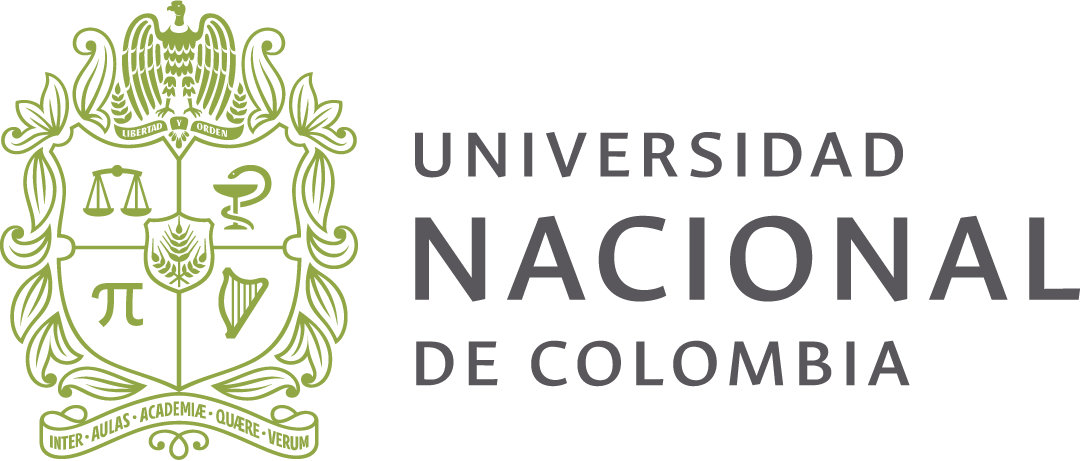
\includegraphics[height=1.5cm]{imagenes/unal_actores.png}\hspace{0.8cm}

\includegraphics[height=1.5cm]{imagenes/univalle_actores.png}\hspace{0.8cm}

\includegraphics[height=1.5cm]{imagenes/cenicafe_fnc_actores.png}\hspace{0.8cm}
\raisebox{9pt}{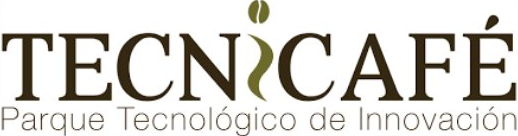
\includegraphics[height=0.82cm]{imagenes/tecnicafe_actores.png}}

\caption{Actores estratégicos del Sistema Nacional de Ciencia, Tecnología e Innovación vinculados al proyecto.}
\end{figure}
